\part{HPC and Exascale}
\chapter*{Introduction}

%%%%%%%%%%%%%%%%%%%%%%%%%%%%%%%%%%%%%%%%%%%%%%%%%%%%%%%%%%%%%%%%%%%%%
%																	%
%	CHAPTER ONE, THEORY of HPC										%
%																	%
%%%%%%%%%%%%%%%%%%%%%%%%%%%%%%%%%%%%%%%%%%%%%%%%%%%%%%%%%%%%%%%%%%%%%

\chapter{Theory of HPC and performaces}

The general idea of parallelism is to achieve performance. 
And thus we need to define what performance imply in HPC. 
- Reducing total time = Latency 
- Reducing rate of task = Throughput 
- Reducing 

\section{Introduction}
The world of nowaday HPC is managed by some fondamental rules that gives the main direction in the researches. 
This first chapter will present the different laws and rules that comes from HPC theory and observations. 


\section{Speedup, efficiency and scalability}


\subsection{Speedup and efficiency}
Calling latency the time to computer a time, unit of time. 
The latency is define as the time for number
The lower latency is better. 

Considering $n$ the number of processes and $n=1$ the sequential case.
And $T_n$ the execution time with $n$ processes and $T_1$ the sequential one. 
The speedup can be defined using the latency by the formula: 
\begin{equation}
\text{speedup} = S_n =  \frac{T_1}{T_n}
\end{equation}

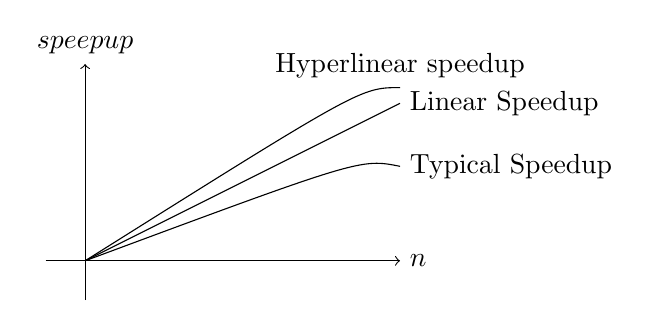
\begin{tikzpicture}
  \draw[->] (-.5,0) -- (4,0) node[right] {$n$};
  \draw[->] (0,-.5) -- (0,2.5) node[above] {$speepup$};
  \draw (0,0) -- (4,2) node[right] {\text{Linear Speedup}};
  \draw (0,0) .. controls (3.5,1.3) .. (4.,1.2) node[right] {\text{Typical Speedup}} ;
  \draw (0,0) .. controls (3.5,2.2) .. (4.,2.2) node[above] {\text{Hyperlinear speedup}} ;
\end{tikzpicture}

And the efficiency is defined by the speedup devided by the number of workers: 
\begin{equation}
\text{efficiency} = \frac{S_n}{n} = \frac{T_1}{nT_n}
\end{equation}

Is the algorithm executes $P$ times faster using $P$ processes, it is then called $superlinear$

\subsection{Scalability}

\section{Amdhal's and Gustafson's law}

The Amdhal's and Gustafson's law show us how to be able to evaluate the maximal available speedup for an application taking in account different characteristics. 

\subsection{Amdahl's law}

The Amdahl's law\cite{amdahl1967validity} is use to find the theoretical speedup in latency of a program.
We can separate a program in two parts, the one that can be execute in parallel and the one that is sequential. 
And even if we reduce the parallel part to infinite the sequential part will reach 100\% of the total time. 

Extracted from the Amdahl paper the law can be writen as: 

\begin{equation}
Speedup = \frac{1}{Seq + \frac{Par}{n}}
\end{equation}

Where $Seq + Par = 1$ and $Seq$ and $Par$ respectively the sequential and parallel ratio of a program. 

\subsection{Gustafson's law}

\section{Flynn taxonomy and executions models}

A right characterization of what a sequential and a parallel machine provide is essential in order to be able to target the architecture in the way they are built.
The flynn taxonomy presents a hierarchical organization of computation machine and executions models.
In this classification \cite{flynn1972some}, Michael J. Flynn present the SIMD,SISI, MISD and MIMD.

\begin{center}
\begin{tabular}{| l | l | l |}
						& Single Data (SD) 	& Multiple Data (MD) \\
\hline
Single Instruction (SI)		&  SISD			& SIMD \\
\hline
Multiple Instructions (MI) 	& 	MISD		& MIMD \\
\hline
\end{tabular}
\end{center}

\subsection{Single Instruction, Single Data: SISD}
This is the model corresponding to a single core CPU with no data parallelism. 
This sequential model is one instruction operate on one data which is then store and the process continue over. 

\subsection{Single Instruction, Multiple Data: SIMD}
This is the execution model corresponding to a many-core architecture like a GPU. 
In the same clock, the same operation is executed on every process on different data. 
The best example stay the work on matrices like a stencil. 

\subsection{Multiple Instructions, Multiple Data: MIMD}

\subsection{Multiple Instructions, Single Data: MISD}
This last model can correspond to a pipeline but even in this case the data are modified after every operations. 

\section{Memory models}
The most common memory models for shared memory are: 
\subsection{UMA}
\subsection{NUMA}
\subsection{COMA}

\subsection{DRAM and PRAM}

\section{Conclusions}

%%%%%%%%%%%%%%%%%%%%%%%%%%%%%%%%%%%%%%%%%%%%%%%%%%%%%%%%%%%%%%%%%%%%%
%																	%
%	CHAPTER TWO, HARDWARE IN HPV									%
%																	%
%%%%%%%%%%%%%%%%%%%%%%%%%%%%%%%%%%%%%%%%%%%%%%%%%%%%%%%%%%%%%%%%%%%%%
\chapter{Hardware in HPC}

\section{Introduction}

\section{Architectures}
\subsection{Classical CPU}

Talk about the ARM architecture 

\subsection{GPGPU}

GPUs are based on the SIMD model of the Flynn taxonomy presented previously, \emph{Single Instruction, Multiple Data}.
The specific execution model is called SIMT (\emph{Single Instruction, Multiple Thread}). It enables the execution of millions of coordinated threads in a data-parallel mode. 
Two main companies provide GPGPUs for the HPC world NVIDIA and AMD, we will present them in that order and conclude on the differences. 

\subsubsection{NVIDIA GPU architecture}

The NVIDIA company was fonded in April 1993 in Santa Clara, Carolina, by three persons in which Jensen Huang, the actual CEO.
Its name seems to come from \textit{invidia} the latin word for Envy and vision, for the graphics generation. 

Known as the pioner in graphics, cryptocurrency, portable devices and now AI, it seems to be even the creator of the name "GPU".
It GPU, inspired from visualisation and gaming at a first glance, is available as a dedicated device  since the Tesla. 
The public GPUs can also be use for dedicated computation but does not feature eMMC memory, double precision or special functions/FFT cores. 

We will describe here the Kepler architecture, this is the one we worked

\begin{figure*}[t!]
\centering
\setlength\fboxsep{0pt}
\setlength\fboxrule{0.25pt}
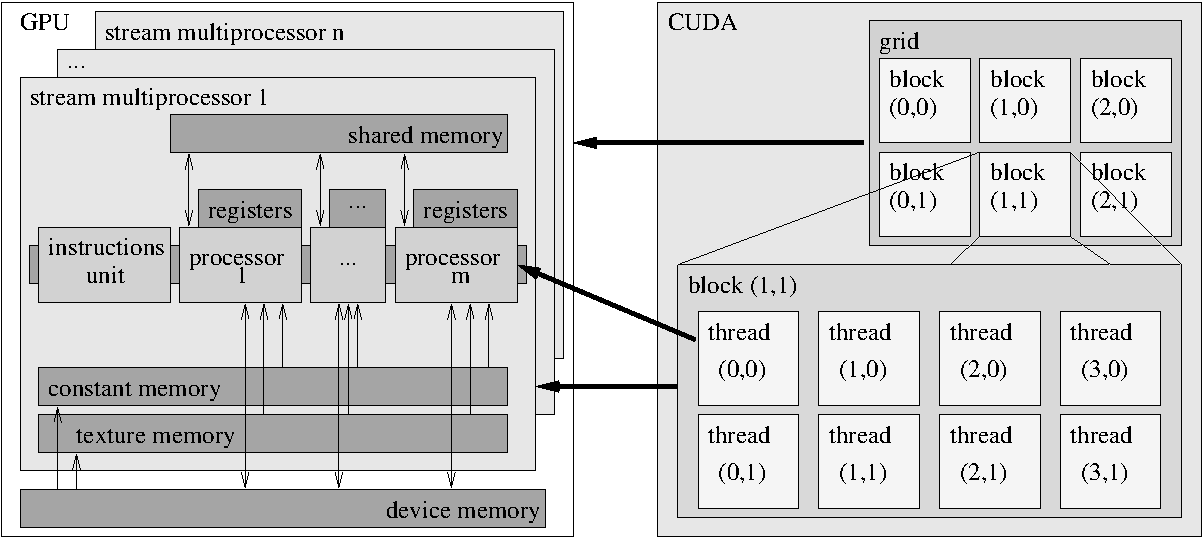
\includegraphics[scale=0.6]{figures/chap1/smx}
\caption{NVIDIA GPU and CUDA architecture overview}
 \label{fig:gpu}
%\vspace{-0.8cm} 
\end{figure*}

As presented in Fig.\ref{fig:gpu}, NVIDIA GPUs include many \emph{Streaming Multiprocessors} (SM), each of which is composed of many \emph{Streaming Processors} (SP). In the Kepler architecture, the SM new generation is called SMX.
%
%In the CUDA programing model~\cite{cuda}, the GPU works as a SIMT co-processor of a conventional CPU. 
Grouped into \emph{blocks}, \textit{threads} execute \emph{kernel} functions synchronously.
Threads within a block can cooperate by sharing data on an SMX and synchronizing their execution to coordinate memory accesses; inside a block, the scheduler organizes \emph{warps} of 32 threads which execute the instructions simultaneously.
The blocks are distributed over the GPU SMXs to be executed independently.

\subsubsection{Memory, bandwidth and streams:}

In order to use data in a CUDA kernel, it has to be first created on the CPU, allocated on the GPU and then transferred from the CPU to the GPU; after the kernel execution, the results have to be transferred back from the GPU to the CPU. 
GPUs consist of several memory categories, organized hierarchically and differing by size, bandwidth and latency.   
On the one hand, the device's main memory is relatively large but has a slow access time due to a huge latency. 
On the other hand, each SMX has a small amount of shared memory and L1 cache, accessible by its SPs, with faster access, and registers organized as an SP-local memory. 
SMXs also have a constant memory cache and a texture memory cache.
%, that are linked to the constant and texture memories physically located in the device memory: these are read-only and have faster access time than the rest of the memory categories.
Reaching optimal computing efficiency requires considerable effort while programming.
Most of the global memory latency can then be hidden by the threads scheduler if there is enough computational effort to be executed while waiting for the global memory access to complete. Another way to hide this latency is to use streams to overlap kernel computation and memory load. 

\subsubsection{Threads synchronization:}
It is also important to note that branching instructions may break the threads synchronous execution inside a warp and thus affect the program efficiency. 
This is the reason why test-based applications, like combinatorial problems that are inherently irregular, are considered as bad candidates for GPU implementation. 
%This is particularly true with regard to combinatorial problems resolution. 
Thus we intend to provide a way to regularize their execution, in order to get good acceleration with GPU computation. 

\subsection{FPGA and ASICS}

\section{Clusters and interconnection}
\subsection{TOP500 remarquable clusters}
\subsubsection{Sunway Taihulight}

This is the third Chinese supercomputer to be ranked in the first position of the TOP500 list. (VERIFIER INFO)
A recent report from Jack Dongarra, a figure in HPC, decrypt all the architecture of this supercomputer\cite{dongarra2016report}. 
The most interessant point is the conception of this machine, completely done in China. 
The Sunway CPUs were invented and built in China and have a specific architecture. 


\subsubsection{Titan}
\subsubsection{K-Computer}
\subsubsection{Sequoia}
\section{ROMEO Supercomputer}

\begin{equation}
\frac{1}{sin(x)}
\end{equation}

%%%%%%%%%%%%%%%%%%%%%%%%%%%%%%%%%%%%%%%%%%%%%%%%%%%%%%%%%%%%%%%%%%%%%
%																	%
%	CHAPTER THREE, SOFTWARE AND API									%
%																	%
%%%%%%%%%%%%%%%%%%%%%%%%%%%%%%%%%%%%%%%%%%%%%%%%%%%%%%%%%%%%%%%%%%%%%
\chapter{Software and Benchmarks}

\section{Sofware/API}
\subsection{OpenMP}
\subsection{MPI}
\subsection{CUDA}
\subsection{Charm++}
\subsection{Legion}
\section{Benchmark}
\subsection{TOP500}
\subsection{GRAPH500}
\subsection{GRENN500}

\chapter*{Conclusion}
